% tutorial_example_osem.tex — worked example: MLEM vs OSEM (acceleration) and,
% on the same phantom with resolution switched on, semi-convergence and early
% stopping. Standalone; reuses recocrysp_tutorial.sty and the shared bibliography.
% Refers to the Foundations tutorial (Part I) by name. Code: tutorial/examples/osem/.
\documentclass[11pt,a4paper]{article}
\usepackage{recocrysp_tutorial}

\title{RecoCrysp Tutorial\,---\,Worked Example\\[2pt]
       \large Acceleration and Early Stopping: MLEM vs OSEM}
\author{J.~J.~G\'omez-Cadenas}
\date{\today}

\begin{document}
\maketitle

\begin{abstract}
A worked example in two acts on one phantom --- the Derenzo-in-water of the
Resolution example --- holding the physics fixed and changing only the
reconstruction. The first act reconstructs \emph{sharp} data with MLEM and with
ordered-subsets EM (OSEM) at several subset counts, showing that one OSEM update
equals one MLEM iteration and that $M$ subsets reach the same image about $M$
times faster --- at a small accuracy cost as $M$ grows. The second act switches on
the $5\,\mathrm{mm}$ detector resolution and finds the thing the sharp data
\emph{refused} to show: with a band-limited target the error against $\Gop\xv$
dips and then climbs, so the reconstruction must be stopped early. Code in
\code{tutorial/examples/osem/}.
\end{abstract}

\section{Overview}
\label{sec:ex-osem:overview}

The Foundations tutorial derived two reconstruction ideas that this example puts
on screen: OSEM, which accelerates MLEM by updating the image once per subset of
events (Part~I, Acceleration and Noise), and \emph{semi-convergence}, the fact
that MLEM run to convergence overfits Poisson noise and is best stopped early
(same section). Both are properties of the \emph{solver}, not the data, so we fix
one phantom, one geometry, one attenuation map, and one sensitivity image, and
change only how we iterate.

The two acts are deliberately a matched pair. Act~1 uses sharp data ($\Gop=\mathbf
I$) and asks how \emph{fast} we can reconstruct; act~2 uses smeared data and asks
\emph{when to stop}. The link between them is a small discovery made while
building the example, told in Section~\ref{sec:ex-osem:act2}: the sharp data of
act~1 will not exhibit semi-convergence at all, and understanding why is what
makes the resolution case in act~2 inevitable.

\section{Setup}
\label{sec:ex-osem:setup}

The phantom, scanner, attenuation and sensitivity are those of the Resolution
example: a Derenzo rod phantom inside a water cylinder of radius $80\,\mathrm{mm}$
on the CRYSP continuous scanner ($\varnothing\,77.4\,\mathrm{cm}$, AFOV
$102.4\,\mathrm{cm}$). The grid is a $1.5\,\mathrm{mm}$ isotropic
$121\times121\times71$ volume --- coarser than the Resolution example, since here
we compare solvers rather than chase the finest rods. Geometry, attenuation
$\att=\exp(-\Aop\bm\mu)$ and the sensitivity image $\sensv=\Aadj(\att)$ are built
once and shared by every reconstruction in both acts:
\begin{lstlisting}
xs, xe = sample_lors(sc, nlors; rng = MersenneTwister(seed))
a    = exp.(-joseph3d_fwd(xs, xe, mumap, org, vs))        # attenuation
sens = sensitivity_image(xs, xe, n, org, vs; weights = a) # A^T(a), shared
x0   = Float32.(sens .> 0)
\end{lstlisting}

To compare solvers fairly we drive the iterations by hand from the public
\code{em\_update} (one MLEM iteration as a preconditioned gradient step, Part~I)
and time only the solve, evaluating the error and likelihood outside the timed
region. One MLEM step updates the image once from all events; one OSEM
\emph{epoch} updates it once per subset, so an epoch of $M$ subsets does about the
same projection work as a single MLEM iteration while advancing the image $M$
times:
\begin{lstlisting}
for k in 1:niter                       # MLEM: one update per step
    t += @elapsed (x = em_update(model, x))
end

models = subset_models(xs, xe, org, vs, n, M; counts = counts, mult = a)
for e in 1:nepochs                     # OSEM: one epoch = M updates
    t += @elapsed for m in models
        x = em_update(m, x)            # each subset has its own subset sensitivity
    end
end
\end{lstlisting}
Here \code{subset\_models} splits the event list into $M$ interleaved subsets,
each carrying its own exact subset sensitivity $\Aadj_{(m)}(\att)$, exactly the
construction of Part~I.

\section{Act 1\,---\,acceleration on sharp data}
\label{sec:ex-osem:act1}

The first dataset is sharp: $\pred=\att\odot(\Aop\xv_{\mathrm{true}})$, Poisson
sampled at $1.5\times10^{7}$ counts over $2\times10^{7}$ LORs. We reconstruct it
with MLEM for $48$ iterations and with OSEM at $M\in\{4,8,16\}$ subsets, each for
$48/M$ epochs, so all four runs perform the same number of image updates. The
error is measured against the sharp truth, normalized over the rods.

Figure~\ref{fig:osem-act1} tells the story in two axes. Against the
\emph{image-update count} (lower-left) the four curves lie on top of one another:
one OSEM update is worth one MLEM iteration, and the reconstructed images at
matched updates are visually identical (top row). Against \emph{wall-clock}
(lower-right) the OSEM curves are the MLEM curve compressed by $M$: the measured
speed-ups to the same image are $4.0\times$, $8.0\times$ and $15.4\times$ for
$M=4,8,16$, tracking the subset count as expected.

\begin{figure}[t]
  \centering
  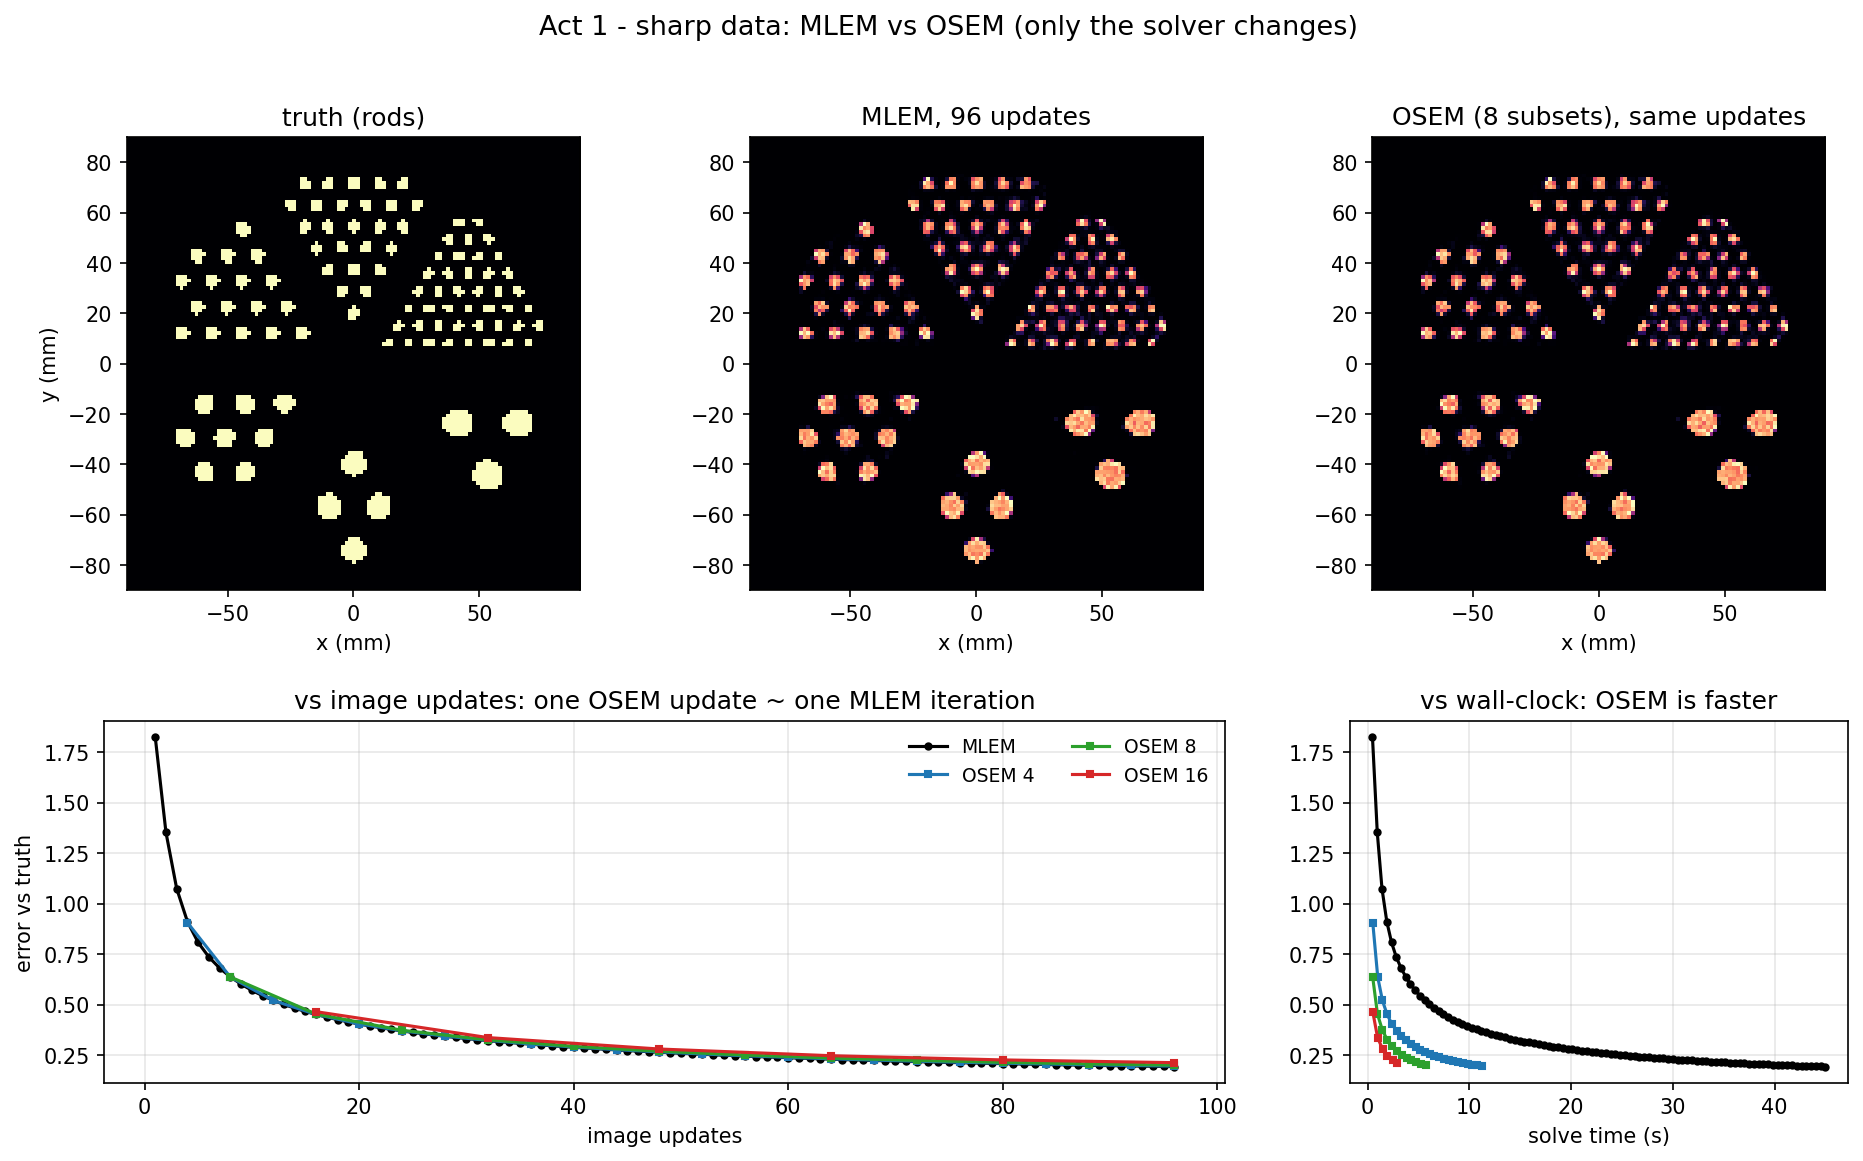
\includegraphics[width=\textwidth]{figures/osem_result.png}
  \caption{Act~1, sharp data. Top: the truth and the MLEM and OSEM ($8$ subsets)
    reconstructions at the same number of image updates --- indistinguishable.
    Bottom-left: error against the truth versus image updates; MLEM and all OSEM
    runs overlay. Bottom-right: the same error versus wall-clock; OSEM-$M$ reaches
    the image about $M$ times sooner. Only the solver changes.}
  \label{fig:osem-act1}
\end{figure}

The acceleration is not quite free, and the example shows the cost. The error
floors come out ordered $0.193$ (MLEM) $<0.195$ (OSEM-4) $<0.200$ (OSEM-8)
$<0.212$ (OSEM-16): more subsets reach a slightly worse final image. This is the
limit cycle of Part~I --- OSEM does not converge to a single point but drifts among
$M$ nearby images, and the drift widens as the counts per subset shrink. A
moderate subset count buys most of the speed at little cost; a large one trades
accuracy for it.

\section{Act 2\,---\,early stopping on smeared data}
\label{sec:ex-osem:act2}

Act~1 left a loose end. Semi-convergence predicts that the error against the
truth should \emph{rise} once MLEM begins fitting noise, yet in
Figure~\ref{fig:osem-act1} it falls monotonically through all $48$ iterations.
The reason is structural: the sharp truth contains detail at every scale --- rod
edges, gaps --- so MLEM keeps making genuine progress for a long time, and that
progress masks the slow growth of noise. The turn is there, but far out of frame.

Switching on the detector resolution removes the masking. With the activity
blurred by the $5\,\mathrm{mm}$ operator $\Gop$ at simulation time, the
reconstruction can recover only $\Gop\xv_{\mathrm{true}}$ --- a \emph{band-limited},
smooth image with nothing finer than the resolution in it. MLEM recovers that
smooth target in a handful of iterations and then has no real structure left to
fit, while its high-frequency noise amplification continues unabated. The
recoverable target is built with the same library operator used in the Resolution
example, and the data are sampled at fewer counts ($7\times10^{6}$) so that noise
asserts itself early:
\begin{lstlisting}
x_blur  = gaussian_blur(x_true, fwhm, vs)               # G x_true (band-limited)
ybar2   = a .* joseph3d_fwd(xs, xe, x_blur, org, vs)
counts2 = [rand(rng, Poisson(l)) for l in scale2 .* ybar2]
\end{lstlisting}

The consequence is semi-convergence, now plainly in view
(Figure~\ref{fig:osem-act2}). The error against $\Gop\xv$ falls to a minimum of
$0.251$ at $26$ updates and then climbs to $0.336$ by $96$: the reconstruction
passes through its best estimate and degrades if pushed further. The images make
it concrete --- the early-stop iterate resembles the recoverable $\Gop\xv$, while
the run-on iterate is visibly grainier as Poisson noise is fitted. The remedy is
\emph{early stopping}: take the image at the minimum. OSEM inherits the behaviour
and reaches the same minimum about $M$ times sooner ($8.6\times$ here for
$M=8$), so the two acts compose --- accelerate with subsets, and stop early.

\begin{figure}[t]
  \centering
  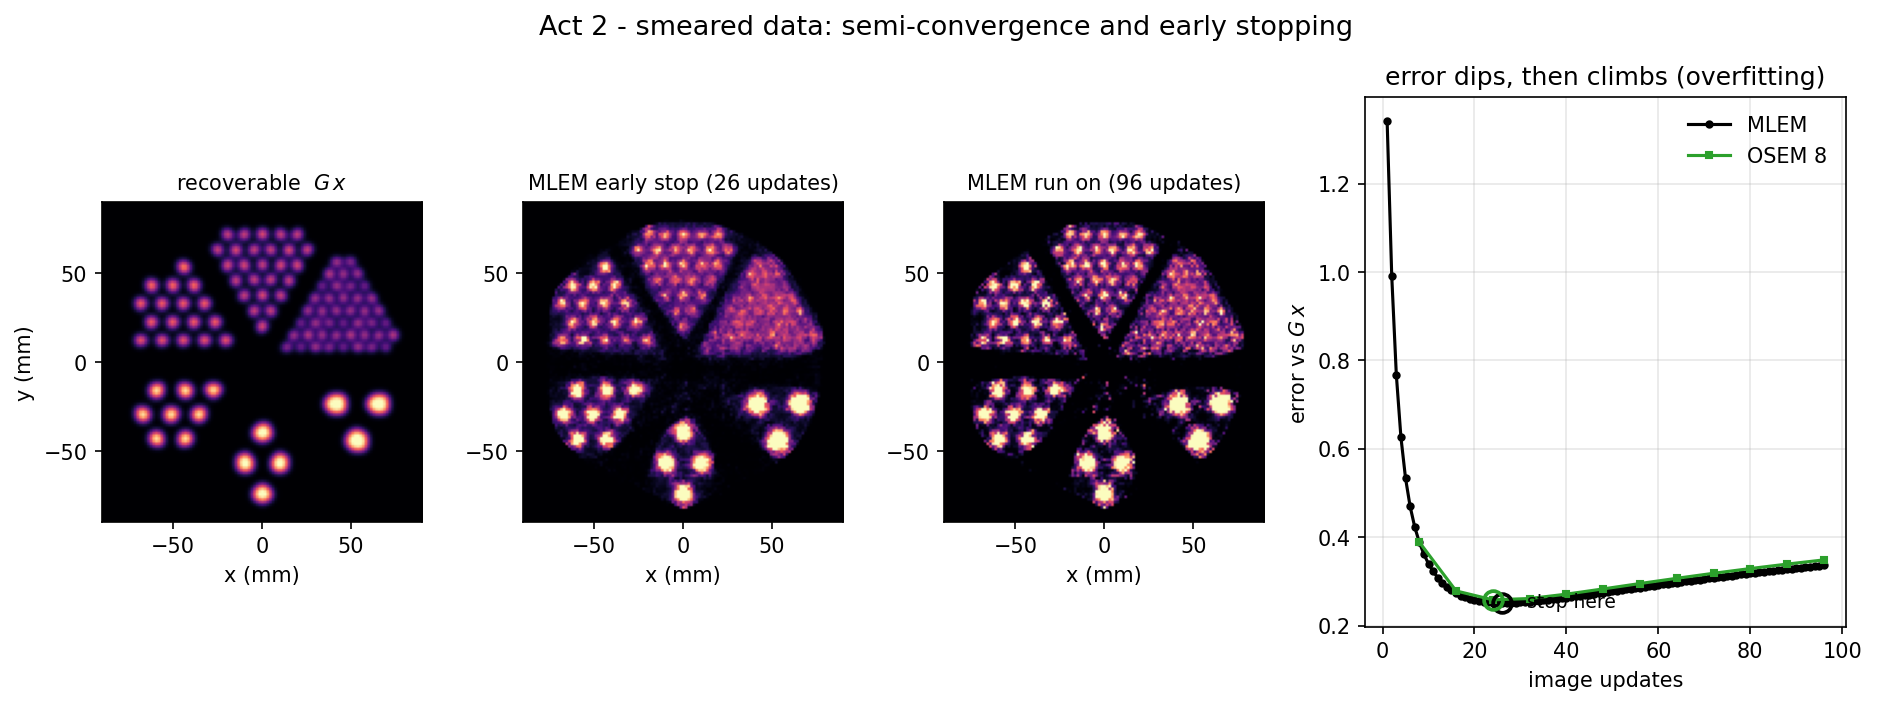
\includegraphics[width=\textwidth]{figures/osem_earlystop_result.png}
  \caption{Act~2, smeared data. From left: the recoverable image $\Gop\xv$; the
    MLEM iterate at the early-stopping minimum ($26$ updates), which resembles it;
    and the run-on iterate ($96$ updates), grainier from fitting noise. Right: the
    error against $\Gop\xv$ dips and then climbs --- semi-convergence --- with each
    solver's minimum marked. OSEM reaches the bottom sooner.}
  \label{fig:osem-act2}
\end{figure}

The two acts use different count levels by design: act~1 wants clean data so the
MLEM/OSEM agreement is unambiguous, act~2 wants noisier data so overfitting bites
within a short run. The turn exists at any count level; fewer counts only bring it
earlier and make it steeper.

\section{Running the example}
\label{sec:ex-osem:run}

The code is in \code{tutorial/examples/osem/}: \code{run.jl}, \code{osem.toml}
(all parameters), \code{osem\_plot.py} (writes both figures). From the repository
root:
\begin{lstlisting}
julia --project=tutorial/examples/osem -e \
  'using Pkg; Pkg.develop(path="."); Pkg.instantiate()'   # first time
julia -t auto --project=tutorial/examples/osem \
  tutorial/examples/osem/run.jl
python3 tutorial/examples/osem/osem_plot.py
\end{lstlisting}
The full configuration is
\begin{lstlisting}
[scanner]
diameter = 774.0
afov     = 1024.0

[grid]
n       = [121, 121, 71]
voxsize = 1.5

[derenzo]
radius        = 80.0
length        = 100.0
rod_diameters = [4.0, 5.0, 6.0, 8.0, 10.0, 12.0]
spacing       = 2.0

[phantom]
mu_water = 0.0096

[resolution]
fwhm = 5.0

[sim]
n_lors         = 20000000
total_counts   = 1.5e7   # act 1 (sharp): clean
smeared_counts = 7.0e6   # act 2 (smeared): noisier, turns over early
seed           = 1

[recon]
niter   = 96
subsets = [4, 8, 16]
m_show  = 8
\end{lstlisting}
Lower \code{n\_lors} or raise \code{voxsize} to run lighter; the run is two full
sweeps of reconstructions and takes a few minutes.

\section{What this shows}
\label{sec:ex-osem:next}

The reconstruction code is unchanged from the earlier examples; only the schedule
of updates differs. OSEM delivers an $M$-fold acceleration at the price of a
slightly biased limit cycle, and semi-convergence makes early stopping a
necessity rather than an option once the recoverable image is band-limited ---
which, with any real detector resolution, it always is. Together with attenuation
(first example) and resolution (second example), the solver behaviour here
completes the reconstruction half of the picture; the remaining work is the
additive backgrounds, scatter and randoms, entering through the
\code{contamination} field in the examples that follow~\cite{crysp2026}.

% tbsrc/references.tex — bibliography (self-contained, no bibtex step).
\begin{thebibliography}{9}

\bibitem{joseph1982}
P.~M. Joseph,
\emph{An improved algorithm for reprojecting rays through pixel images},
IEEE Trans.\ Med.\ Imaging \textbf{1}(3):192--196, 1982.

\bibitem{shepp1982}
L.~A. Shepp and Y.~Vardi,
\emph{Maximum likelihood reconstruction for emission tomography},
IEEE Trans.\ Med.\ Imaging \textbf{1}(2):113--122, 1982.

\bibitem{lange1984}
K.~Lange and R.~Carson,
\emph{EM reconstruction algorithms for emission and transmission tomography},
J.\ Comput.\ Assist.\ Tomogr.\ \textbf{8}(2):306--316, 1984.

\bibitem{hudson1994}
H.~M. Hudson and R.~S. Larkin,
\emph{Accelerated image reconstruction using ordered subsets of projection
data},
IEEE Trans.\ Med.\ Imaging \textbf{13}(4):601--609, 1994.

\bibitem{watson2000}
C.~C. Watson,
\emph{New, faster, image-based scatter correction for 3D PET},
IEEE Trans.\ Nucl.\ Sci.\ \textbf{47}(4):1587--1594, 2000.

\bibitem{moses2011}
W.~W. Moses,
\emph{Fundamental limits of spatial resolution in PET},
Nucl.\ Instrum.\ Methods Phys.\ Res.\ A \textbf{648}:S236--S240, 2011.

\bibitem{schramm2024}
G.~Schramm and K.~Thielemans,
\emph{PARALLELPROJ---an open-source framework for fast calculation of
projections in tomography},
Front.\ Nucl.\ Med.\ \textbf{3}:1324562, 2024.

\end{thebibliography}


\end{document}
